\documentclass[11pt,letterpaper]{article}
\usepackage[utf8]{inputenc}
\usepackage[margin=0.9in]{geometry}
\usepackage{tikz}
\usetikzlibrary{shapes.geometric, arrows.meta, positioning, calc, shadows, fit, backgrounds}
\usepackage{booktabs}
\usepackage{longtable}
\usepackage{xcolor}
\usepackage{hyperref}
\usepackage{fancyhdr}
\usepackage{enumitem}
\usepackage{multicol}
\usepackage{tcolorbox}

% Colors
\definecolor{asuscolor}{RGB}{0, 102, 179}
\definecolor{tendacolor}{RGB}{255, 102, 0}
\definecolor{routercolor}{RGB}{52, 73, 94}
\definecolor{tvcolor}{RGB}{155, 89, 182}
\definecolor{computercolor}{RGB}{41, 128, 185}
\definecolor{printercolor}{RGB}{39, 174, 96}
\definecolor{voipcolor}{RGB}{230, 126, 34}
\definecolor{iotcolor}{RGB}{241, 196, 15}
\definecolor{mobilecolor}{RGB}{231, 76, 60}
\definecolor{warningcolor}{RGB}{231, 76, 60}
\definecolor{goodcolor}{RGB}{39, 174, 96}
\definecolor{networkcolor}{RGB}{52, 152, 219}
\definecolor{bridgecolor}{RGB}{142, 68, 173}

\tcbuselibrary{skins,breakable}

\pagestyle{fancy}
\fancyhf{}
\rhead{Network Mega Guide}
\lhead{Nathan's Home Network}
\rfoot{Page \thepage}
\setlength{\headheight}{14pt}

\title{\textbf{Network Mega Guide}\\[0.5em]\large Complete Analysis of Home Network Infrastructure\\[0.3em]\normalsize Superdooper 5G + Test Networks}
\author{Generated by Claude Code with WireMCP}
\date{\today}

\begin{document}

\maketitle

\begin{tcolorbox}[colback=blue!5,colframe=blue!50!black,title=Quick Reference]
\begin{multicols}{2}
\textbf{Network 1: Superdooper 5G}
\begin{itemize}[noitemsep]
    \item Subnet: 192.168.50.0/24
    \item Router: ASUS RT-AX3000
    \item Gateway: 192.168.50.1
    \item WiFi: 802.11ax (WiFi 6)
    \item Devices: 14
\end{itemize}
\columnbreak
\textbf{Network 2: Test}
\begin{itemize}[noitemsep]
    \item Subnet: 192.168.2.0/24
    \item Router: Tenda
    \item Gateway: 192.168.2.1
    \item WiFi: 802.11ac (WiFi 5)
    \item Devices: 5
\end{itemize}
\end{multicols}
\end{tcolorbox}

\tableofcontents
\newpage

%==============================================================================
\section{Network Overview}
%==============================================================================

This guide documents two separate WiFi networks that can be bridged for extended coverage:

\subsection{Network Architecture}

\begin{center}
\begin{tikzpicture}[
    network/.style={rectangle, rounded corners, draw=#1, fill=#1!15,
                   thick, minimum width=4cm, minimum height=2cm, drop shadow},
    router/.style={rectangle, rounded corners, draw=#1, fill=#1!25,
                   thick, minimum width=2.5cm, minimum height=1cm},
    bridge/.style={rectangle, rounded corners, draw=bridgecolor, fill=bridgecolor!20,
                   thick, dashed, minimum width=2cm, minimum height=0.8cm},
    arrow/.style={->, >=Stealth, thick, gray}
]

% Internet
\node[draw, cloud, cloud puffs=12, cloud puff arc=120, aspect=3,
      minimum width=4cm, minimum height=1.5cm, fill=blue!10]
      (internet) at (0,4) {\textbf{Internet}};

% Primary Network (Superdooper)
\node[network=asuscolor] (superdooper) at (-4,1) {};
\node[router=asuscolor] at (-4,1.5) {\textbf{ASUS RT-AX3000}};
\node[font=\small] at (-4,0.5) {192.168.50.0/24};
\node[font=\footnotesize, asuscolor] at (-4,0) {\textit{Superdooper 5G}};

% Secondary Network (Test)
\node[network=tendacolor] (test) at (4,1) {};
\node[router=tendacolor] at (4,1.5) {\textbf{Tenda Router}};
\node[font=\small] at (4,0.5) {192.168.2.0/24};
\node[font=\footnotesize, tendacolor] at (4,0) {\textit{Test}};

% Bridge possibility
\node[bridge] (bridge) at (0,0) {Bridge?};

% Connections
\draw[arrow, very thick] (internet) -- (-2,2.5) -- (superdooper);
\draw[arrow, very thick] (internet) -- (2,2.5) -- (test);
\draw[arrow, dashed, bridgecolor] (superdooper) -- (bridge);
\draw[arrow, dashed, bridgecolor] (test) -- (bridge);

% Device counts
\node[font=\footnotesize, fill=white] at (-4,-1.2) {14 devices};
\node[font=\footnotesize, fill=white] at (4,-1.2) {5 devices};

\end{tikzpicture}
\end{center}

\subsection{Network Comparison}

\begin{center}
\begin{tabular}{lcc}
\toprule
\textbf{Feature} & \textbf{Superdooper 5G} & \textbf{Test} \\
\midrule
Router Brand & ASUS & Tenda \\
Router Model & RT-AX3000 & Unknown \\
Subnet & 192.168.50.0/24 & 192.168.2.0/24 \\
Gateway IP & 192.168.50.1 & 192.168.2.1 \\
WiFi Standard & 802.11ax (WiFi 6) & 802.11ac (WiFi 5) \\
Channel & 36 (5GHz) & 36 (5GHz) \\
Signal Strength & -63 dBm & -57 dBm \\
SNR & 25 dB & 32 dB \\
Max Speed & 648 Mbps & 585 Mbps \\
Latency to Gateway & 2.3 ms & 3.4 ms \\
Packet Loss & 0\% & 0\% \\
Total Devices & 14 & 5 \\
\bottomrule
\end{tabular}
\end{center}

%==============================================================================
\section{Network 1: Superdooper 5G (Primary)}
%==============================================================================

\begin{tcolorbox}[colback=asuscolor!5,colframe=asuscolor,title=Superdooper 5G Network Summary]
\textbf{Status:} \textcolor{goodcolor}{Healthy} | \textbf{Router:} ASUS RT-AX3000 | \textbf{Subnet:} 192.168.50.0/24
\end{tcolorbox}

\subsection{Network Topology}

\begin{center}
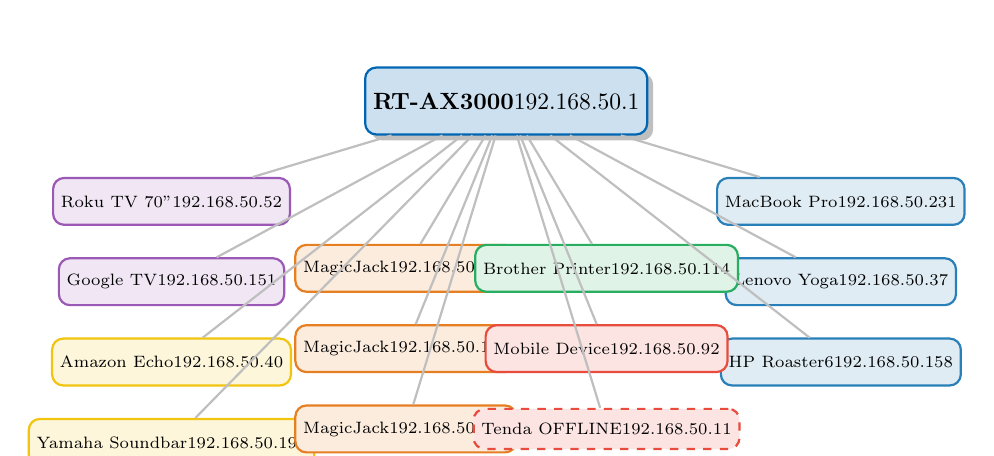
\begin{tikzpicture}[scale=0.85, transform shape,
    router/.style={rectangle, rounded corners, draw=asuscolor, fill=asuscolor!20,
                   thick, minimum width=2.8cm, minimum height=1cm, drop shadow},
    device/.style={rectangle, rounded corners, draw=#1, fill=#1!15,
                   thick, minimum width=2.2cm, minimum height=0.7cm, font=\scriptsize},
    extender/.style={rectangle, rounded corners, draw=warningcolor, fill=warningcolor!15,
                     thick, dashed, minimum width=2cm, minimum height=0.6cm, font=\scriptsize},
    connection/.style={-, thick, gray!50}
]

% Router
\node[router] (router) at (0,0) {\textbf{RT-AX3000}\\192.168.50.1};

% Left side - Entertainment
\node[device=tvcolor] (roku) at (-5,-1.5) {Roku TV 70"\\192.168.50.52};
\node[device=tvcolor] (gtv) at (-5,-2.7) {Google TV\\192.168.50.151};
\node[device=iotcolor] (echo) at (-5,-3.9) {Amazon Echo\\192.168.50.40};
\node[device=iotcolor] (sound) at (-5,-5.1) {Yamaha Soundbar\\192.168.50.195};

% Center - VoIP
\node[device=voipcolor] (v1) at (-1.5,-2.5) {MagicJack\\192.168.50.124};
\node[device=voipcolor] (v2) at (-1.5,-3.7) {MagicJack\\192.168.50.150};
\node[device=voipcolor] (v3) at (-1.5,-4.9) {MagicJack\\192.168.50.201};

% Right side - Computers
\node[device=computercolor] (mac) at (5,-1.5) {MacBook Pro\\192.168.50.231};
\node[device=computercolor] (yoga) at (5,-2.7) {Lenovo Yoga\\192.168.50.37};
\node[device=computercolor] (hp) at (5,-3.9) {HP Roaster6\\192.168.50.158};

% Other
\node[device=printercolor] (printer) at (1.5,-2.5) {Brother Printer\\192.168.50.114};
\node[device=mobilecolor] (mobile) at (1.5,-3.7) {Mobile Device\\192.168.50.92};
\node[extender] (tenda) at (1.5,-4.9) {Tenda OFFLINE\\192.168.50.11};

% Connections
\foreach \n in {roku,gtv,echo,sound,v1,v2,v3,mac,yoga,hp,printer,mobile,tenda}
    \draw[connection] (router) -- (\n);

\end{tikzpicture}
\end{center}

\subsection{Device Inventory}

\begin{longtable}{@{}lllll@{}}
\toprule
\textbf{IP} & \textbf{MAC Address} & \textbf{Vendor} & \textbf{Type} & \textbf{Name} \\
\midrule
\endhead
.1 & f0:2f:74:6e:5b:f8 & ASUS & Router & RT-AX3000-5BF8 \\
.11 & c8:3a:35:3a:c2:35 & Tenda & Extender & \textcolor{warningcolor}{OFFLINE} \\
.37 & 14:ac:60:33:f6:51 & Lenovo & Laptop & TG-Yoga \\
.40 & 48:b4:23:35:30:25 & Amazon & IoT & Echo/Fire \\
.52 & f0:a3:b2:b3:14:fd & Roku & Smart TV & 70" onn Roku TV \\
.92 & 16:cb:af:68:84:dd & Private & Mobile & Unknown \\
.114 & 00:80:92:d6:6a:99 & Brother & Printer & MFC-L8850CDW \\
.124 & 6c:33:a9:70:8d:75 & MagicJack & VoIP & Phone 1 \\
.150 & 6c:33:a9:7b:6b:5e & MagicJack & VoIP & Phone 2 \\
.151 & 02:58:a5:5a:ac:2a & Private & Smart TV & GoogleTV9356 \\
.158 & dc:4a:3e:79:bb:7f & HP & Computer & Roaster6 \\
.195 & 00:22:6c:18:e2:72 & Yamaha & Audio & ATS-1090 \\
.201 & 6c:33:a9:3e:20:48 & MagicJack & VoIP & Phone 3 \\
.231 & 06:fe:91:16:fb:2d & Apple & Computer & MacBook Pro \\
\bottomrule
\end{longtable}

\subsection{Issues Detected}

\begin{tcolorbox}[colback=warningcolor!10,colframe=warningcolor,title=Warning: Tenda Device Offline]
\textbf{Device:} 192.168.50.11 (c8:3a:35:3a:c2:35)\\
\textbf{Status:} 100\% packet loss - completely unresponsive\\
\textbf{Impact:} If this is a range extender, it may cause roaming issues when it intermittently reconnects.\\
\textbf{Action:} Locate and remove or replace this device.
\end{tcolorbox}

%==============================================================================
\section{Network 2: Test (Secondary)}
%==============================================================================

\begin{tcolorbox}[colback=tendacolor!5,colframe=tendacolor,title=Test Network Summary]
\textbf{Status:} \textcolor{goodcolor}{Healthy} | \textbf{Router:} Tenda | \textbf{Subnet:} 192.168.2.0/24
\end{tcolorbox}

\subsection{Network Topology}

\begin{center}
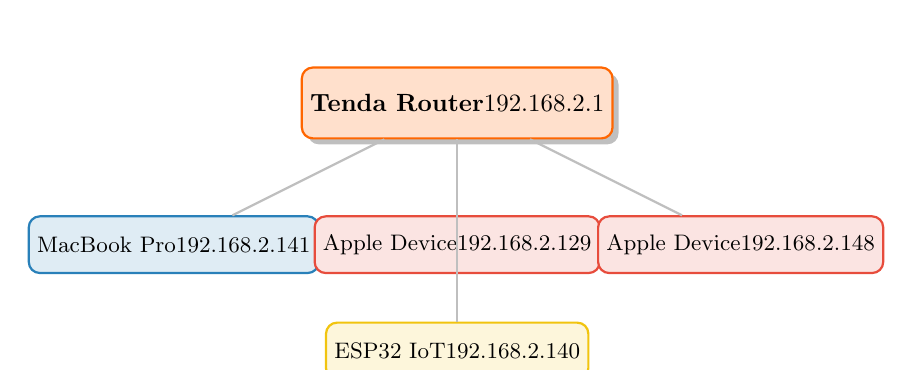
\begin{tikzpicture}[scale=0.9, transform shape,
    router/.style={rectangle, rounded corners, draw=tendacolor, fill=tendacolor!20,
                   thick, minimum width=2.8cm, minimum height=1cm, drop shadow},
    device/.style={rectangle, rounded corners, draw=#1, fill=#1!15,
                   thick, minimum width=2.4cm, minimum height=0.8cm, font=\small}
]

% Router
\node[router] (router) at (0,0) {\textbf{Tenda Router}\\192.168.2.1};

% Devices
\node[device=computercolor] (mac) at (-4,-2) {MacBook Pro\\192.168.2.141};
\node[device=mobilecolor] (apple1) at (0,-2) {Apple Device\\192.168.2.129};
\node[device=mobilecolor] (apple2) at (4,-2) {Apple Device\\192.168.2.148};
\node[device=iotcolor] (esp) at (0,-3.5) {ESP32 IoT\\192.168.2.140};

% Connections
\foreach \n in {mac,apple1,apple2,esp}
    \draw[-, thick, gray!50] (router) -- (\n);

\end{tikzpicture}
\end{center}

\subsection{Device Inventory}

\begin{center}
\begin{tabular}{@{}lllll@{}}
\toprule
\textbf{IP} & \textbf{MAC Address} & \textbf{Vendor} & \textbf{Type} & \textbf{Notes} \\
\midrule
.1 & c8:3a:35:3a:c2:30 & Tenda & Router & Gateway \\
.129 & 10:ff:e0:4c:d7:4e & Apple & Mobile & iPhone/iPad \\
.140 & 80:3f:5d:6d:2d:5c & Espressif & IoT & ESP32 smart device \\
.141 & c6:71:c7:f0:56:bb & Apple & Computer & MacBook Pro \\
.148 & cc:9e:a2:41:2b:69 & Apple & Mobile & iPhone/iPad \\
\bottomrule
\end{tabular}
\end{center}

\subsection{Traffic Analysis}

\begin{center}
\begin{tabular}{lrr}
\toprule
\textbf{Protocol} & \textbf{Packets} & \textbf{Percentage} \\
\midrule
TCP/TLS (Encrypted) & 2,867 & 98.0\% \\
UDP/QUIC & 54 & 1.8\% \\
ARP & 5 & 0.2\% \\
\bottomrule
\end{tabular}
\end{center}

\textbf{Top Bandwidth Consumer:} 34.36.57.103 (Google Cloud) - 6.6 MB in 30 seconds

%==============================================================================
\section{Bridge Configuration Guide}
%==============================================================================

To bridge the two networks for seamless roaming:

\subsection{Option 1: Wireless Bridge Mode (Recommended)}

Configure the Tenda router as a wireless bridge to the ASUS:

\begin{enumerate}
    \item Access Tenda router at \url{http://192.168.2.1}
    \item Navigate to \textbf{Wireless Settings} $\rightarrow$ \textbf{Wireless Bridge/WDS}
    \item Enable \textbf{Bridge Mode}
    \item Scan for networks and select \textbf{Superdooper 5G}
    \item Enter password: (your WiFi password)
    \item \textbf{Important:} Change Tenda's IP to 192.168.50.x range (e.g., 192.168.50.2)
    \item Disable DHCP on Tenda (let ASUS handle DHCP)
    \item Save and reboot
\end{enumerate}

\textbf{Result:} Both networks will be on 192.168.50.0/24, devices can roam seamlessly.

\subsection{Option 2: Keep Separate Networks}

If you prefer isolation:

\begin{itemize}
    \item \textbf{Superdooper 5G (192.168.50.x):} Main network for most devices
    \item \textbf{Test (192.168.2.x):} Secondary/guest network
    \item Use static routes if inter-network communication is needed
\end{itemize}

\subsection{Option 3: ASUS AiMesh}

Replace Tenda with ASUS-compatible mesh node:

\begin{itemize}
    \item Buy any AiMesh-compatible ASUS router
    \item Configure as AiMesh node via ASUS app
    \item Seamless roaming with single SSID
    \item Centralized management
\end{itemize}

%==============================================================================
\section{WiFi Signal Comparison}
%==============================================================================

\begin{center}
\begin{tabular}{lcc}
\toprule
\textbf{Metric} & \textbf{Superdooper 5G} & \textbf{Test} \\
\midrule
RSSI (Signal) & -63 dBm \textcolor{goodcolor}{Good} & -57 dBm \textcolor{goodcolor}{Good} \\
Noise Floor & -88 dBm & -89 dBm \\
SNR & 25 dB \textcolor{goodcolor}{Good} & 32 dB \textcolor{goodcolor}{Excellent} \\
Channel & 36 (5GHz, 80MHz) & 36 (5GHz, 80MHz) \\
WiFi Standard & 802.11ax (WiFi 6) & 802.11ac (WiFi 5) \\
Max TX Rate & 648 Mbps & 585 Mbps \\
MCS Index & 6 & 7 \\
\bottomrule
\end{tabular}
\end{center}

\begin{tcolorbox}[colback=yellow!10,colframe=yellow!50!black,title=Channel Conflict Warning]
Both networks are on \textbf{Channel 36}. If bridging or using both simultaneously, change one to a different channel (e.g., 149, 153, or 157) to avoid interference.
\end{tcolorbox}

%==============================================================================
\section{Optimization Recommendations}
%==============================================================================

\subsection{For Superdooper 5G (ASUS)}

\begin{enumerate}
    \item \textbf{Remove dead Tenda extender at 192.168.50.11}
    \begin{itemize}
        \item Run: \texttt{sudo arp -d 192.168.50.11}
        \item Physically disconnect the device
    \end{itemize}

    \item \textbf{Change channel from 36 to 149 or 157}
    \begin{itemize}
        \item Reduces interference from Test network
        \item Access router at \url{http://192.168.50.1}
    \end{itemize}

    \item \textbf{Enable QoS for VoIP}
    \begin{itemize}
        \item Prioritize 192.168.50.124, .150, .201 (MagicJack)
        \item Prioritize UDP ports 5060, 10000-20000
    \end{itemize}

    \item \textbf{Set DHCP reservations}
    \begin{itemize}
        \item Static IPs for all permanent devices
        \item Easier troubleshooting and port forwarding
    \end{itemize}
\end{enumerate}

\subsection{For Test (Tenda)}

\begin{enumerate}
    \item \textbf{Change channel to 149 or 157}
    \begin{itemize}
        \item Avoid conflict with Superdooper on channel 36
    \end{itemize}

    \item \textbf{Update firmware}
    \begin{itemize}
        \item Check Tenda website for updates
    \end{itemize}

    \item \textbf{Consider bridge mode}
    \begin{itemize}
        \item If coverage extension is the goal
        \item Simplifies network management
    \end{itemize}
\end{enumerate}

\subsection{General Recommendations}

\begin{enumerate}
    \item \textbf{Use 5GHz when possible}
    \begin{itemize}
        \item Less interference, higher speeds
        \item Enable band steering on both routers
    \end{itemize}

    \item \textbf{Regular monitoring}
    \begin{itemize}
        \item Run monthly network scans
        \item Check for unknown devices
    \end{itemize}

    \item \textbf{Firmware updates}
    \begin{itemize}
        \item Keep both routers updated
        \item Security patches and performance improvements
    \end{itemize}
\end{enumerate}

%==============================================================================
\section{Monitoring Commands Reference}
%==============================================================================

\begin{tcolorbox}[colback=gray!5,colframe=gray!50!black,title=Useful Commands]
\begin{verbatim}
# Check current WiFi network
networksetup -getairportnetwork en0

# See all devices on network
arp -a | grep "192.168"

# Check WiFi signal quality
/System/Library/PrivateFrameworks/Apple80211.framework/\
Versions/Current/Resources/airport -I

# Scan for WiFi networks
/System/Library/PrivateFrameworks/Apple80211.framework/\
Versions/Current/Resources/airport -s

# Capture network traffic (30 seconds)
sudo tshark -i en0 -a duration:30 -qz conv,ip

# Protocol breakdown
sudo tshark -i en0 -a duration:20 -qz io,phs

# Test latency to gateway
ping -c 10 192.168.50.1   # Superdooper
ping -c 10 192.168.2.1    # Test

# Discover mDNS services
dns-sd -B _services._dns-sd._udp local.
\end{verbatim}
\end{tcolorbox}

%==============================================================================
\section{Network Passwords Reference}
%==============================================================================

\begin{tcolorbox}[colback=red!5,colframe=red!50!black,title=Sensitive Information - Keep Secure]
\begin{tabular}{ll}
\textbf{Network} & \textbf{Password} \\
\midrule
Superdooper 5G & Tantyy12 \\
SuperdooperG & Tantyy12 \\
Superdooper & Tantyy12 \\
Test & Tantyy1212 \\
\end{tabular}

\vspace{0.5em}
\textbf{Note:} Store this document securely. Consider changing passwords periodically.
\end{tcolorbox}

%==============================================================================
\section{Troubleshooting}
%==============================================================================

\subsection{Common Issues and Solutions}

\begin{enumerate}
    \item \textbf{Devices dropping off network}
    \begin{itemize}
        \item Check if Tenda extender (.11) is causing roaming issues
        \item Verify channel separation between networks
        \item Check signal strength at device location
    \end{itemize}

    \item \textbf{Slow speeds}
    \begin{itemize}
        \item Run \texttt{tshark} to identify bandwidth hogs
        \item Check for channel congestion
        \item Verify 5GHz connection (not 2.4GHz)
    \end{itemize}

    \item \textbf{Can't connect to network}
    \begin{itemize}
        \item Verify password
        \item Check if MAC filtering is enabled
        \item Restart router
    \end{itemize}

    \item \textbf{VoIP call quality issues}
    \begin{itemize}
        \item Enable QoS for MagicJack devices
        \item Check for packet loss: \texttt{ping -c 100 192.168.50.1}
        \item Prioritize UDP traffic
    \end{itemize}
\end{enumerate}

%==============================================================================
\section{Conclusion}
%==============================================================================

\begin{tcolorbox}[colback=green!5,colframe=green!50!black,title=Network Health Summary]
\begin{multicols}{2}
\textbf{Superdooper 5G:}
\begin{itemize}[noitemsep]
    \item Status: Healthy
    \item Issue: Dead Tenda extender
    \item Action: Remove device at .11
\end{itemize}
\columnbreak
\textbf{Test:}
\begin{itemize}[noitemsep]
    \item Status: Healthy
    \item Issue: Channel conflict
    \item Action: Change to ch. 149+
\end{itemize}
\end{multicols}

\textbf{Overall:} Both networks are functioning well. Primary recommendation is to remove the offline Tenda device from Superdooper network and change WiFi channels to avoid interference.
\end{tcolorbox}

\end{document}
